\documentclass[fleqn,10pt]{wlscirep}
\usepackage[utf8]{inputenc, graphicx}
\usepackage[T1]{fontenc}
\title{Tarea 4 métodos computacionales}

\author[1,*]{Humberto Ariza}

\affil[1]{Universidad de Los Andes, Bogotá D.C., Colombia}


\affil[*]{h.ariza@uniandes.edu.co}

\begin{abstract}
    Métodos Computacionales
    Tarea 4 — 2018–20
\end{abstract}

\begin{document}

\section{ODE}

\begin{figure}
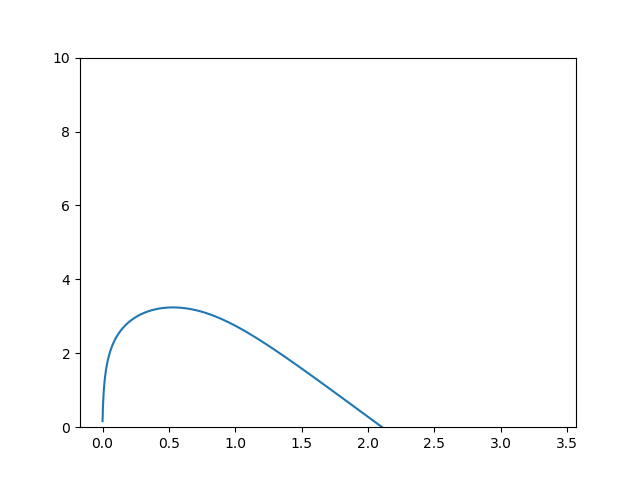
\includegraphics{ODES45.png}
\caption{ODES con 45º}
    

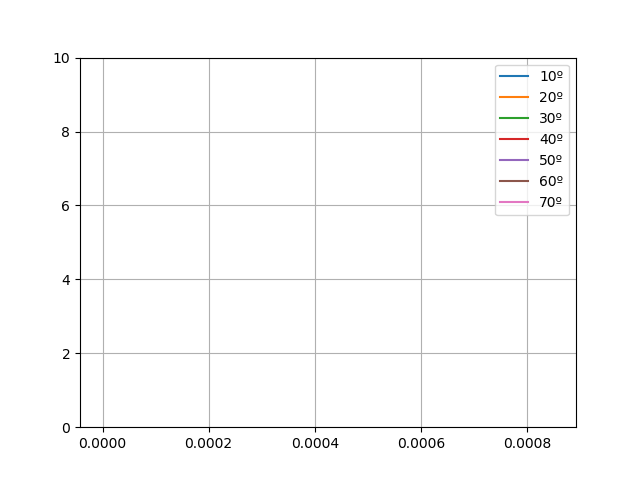
\includegraphics{ODESANGULOS.png}
\caption{ODE CON DIFERENTES ANGULOS}
\end{figure}


\section{PDE}

\end{document}